\immediate\write18{tex penrose.dtx}
\documentclass{ltxdoc}
\usepackage[T1]{fontenc}
\usepackage{trace}
\usepackage{lmodern}
\usepackage{morefloats}
\usepackage[svgnames]{xcolor}
\usepackage{tikz}
\usetikzlibrary{penrose}
\usepackage[numbered]{hypdoc}
\definecolor{lstbgcolor}{rgb}{0.9,0.9,0.9} 
 
\usepackage{listings}
\lstloadlanguages{[LaTeX]TeX}
\lstset{breakatwhitespace=true,breaklines=true,language=TeX}
 
\usepackage{fancyvrb}

\newenvironment{example}
  {\VerbatimEnvironment
   \begin{VerbatimOut}{example.out}}
  {\end{VerbatimOut}
   \begin{center}
   \setlength{\parindent}{0pt}
   \fbox{\begin{minipage}{.9\linewidth}
     \lstset{breakatwhitespace=true,breaklines=true,language=TeX,basicstyle=\small}
     \lstinputlisting[]{example.out}
   \end{minipage}}

   \fbox{\begin{minipage}{.9\linewidth}
     \centering
     \input{example.out}
   \end{minipage}}
\end{center}
}

\colorlet{thinRhombus}{DarkOrchid}
\colorlet{thickRhombus}{DarkSlateGray}
\colorlet{circleArc}{RosyBrown}
\colorlet{longArc}{LawnGreen}

\colorlet{kite}{HotPink}
\colorlet{dart}{Fuchsia}

\colorlet{goldenTriangle}{Gold}
\colorlet{reverseGoldenTriangle}{Magenta}
\colorlet{goldenGnomon}{Cyan}
\colorlet{reverseGoldenGnomon}{LimeGreen}

\makeatletter
\tikzset{
  tint fill colour/.code={%
    \edef\@temp{%
      \def\noexpand\tikz@fillcolor{\tikz@fillcolor!#1}%
      \noexpand\tikz@addoption{\noexpand\pgfsetfillcolor{\tikz@fillcolor!#1}}%
    }%
    \@temp
  }
}
\makeatother

\providecommand*{\url}{\texttt}

\title{The \textsf{Penrose} Package: Documentation}
\author{Andrew Stacey \\ \url{stacey@math.ntnu.no}}
\date{1.0~from 2014/05/07}

\begin{document}
\maketitle

\section{Introduction}

The \textsf{Penrose} package is a TikZ library for drawing Penrose tiles.
Both the kite/dart and rhombus tiles are supported.
There are two main methods for their placement: one that automatically generates a tiling, and one that allows for ``by hand'' placement.
Furthermore, the tiles themselves can be deformed and will still (hopefully!) fit together in the correct fashion.

\section{Initialisation}

To use this package, load the \Verb+tikz+ package and load \Verb+penrose+ as a TikZ library.
Specifically, your preamble should contain:

\begin{verbatim}
\usepackage{tikz}
\usetikzlibrary{penrose}
\end{verbatim}

\section{Usage}

Using this package splits into several components.
There are the two main ways of getting tiles on to the page, and then there are the ways of deforming or styling the tiles once they are there.

\subsection{Placing Tiles ``By Hand''}

It is possible to use the tiles as \Verb+pic+s.
These are mini-drawings introduced in TikZ3.0 that are node-like in style, but a little more geared towards repeatable \emph{drawings} than boxes containing text.
This package defines several \Verb+pic+ types:

\tikzset{
  every Penrose pic/.style={draw,ultra thick},
  every circle arc/.style={draw,thin},
  every long arc/.style={draw,thin},
}

\begin{itemize}
\item Kite \tikz[baseline=-.5ex] \pic[draw,kite];
\item Dart \tikz[baseline=-.5ex] \pic[draw,dart];
\item Thin Rhombus \tikz[baseline=-.5ex] \pic[draw,thin rhombus];
\item Thick Rhombus \tikz[baseline=-.5ex] \pic[draw,thick rhombus];
\item Golden Triangle \tikz[baseline=-.5ex] \pic[draw,golden triangle];
\item Reverse Golden Triangle \tikz[baseline=-.5ex] \pic[draw,reverse golden triangle];
\item Golden Gnomon \tikz[baseline=-.5ex] \pic[draw,golden gnomon];
\item Reverse Golden Gnomon \tikz[baseline=-.5ex] \pic[draw,reverse golden gnomon];
\end{itemize}

The main tiles can have arcs drawn on them to illustrate the matching rules.
The triangles and gnomon are not true Penrose tiles but rather can be used to build tilings so they do not have the arcs.
The two types of each triangle and gnomon are actually different in that they have different matching rules.
This is best illustrated by deforming the paths (see Section~\ref{sec:pathdeform}).

There are two ways in TikZ to specify the \Verb+pic+ type: either as the ``contents'' of the pic or as the argument to the \Verb+pic type+ key.
Each of the tiles comes with a shorthand key which specifies the \Verb+pic type+ and also invokes the key \Verb+every Penrose tile+.
That is, the key \Verb+dart+ calls the \Verb+every Penrose tile+ key and specifies the \Verb+pic type+ as \Verb+dart+.

The tiles can be placed using standard TikZ methods.
One important thing to note is that by default, \Verb+pic+s are like \Verb+nodes+ in that they only respond to ambient translations, and not to rotations and scaling.
To make them notice this, use the key \Verb+transform shape+ or specify the transformation to the \Verb+pic+ directly.
If the shortcut keys are used to specify the tiles, this can be put in the \Verb+every Penrose pic+ style.

TikZ \Verb+pic+s can be named, using the \Verb+name=<name>+ key.
When a Penrose tile has been named then it can be used for positioning other tiles.
Each edge is assigned a label from \Verb+a b c A B C+ and a new tile can be aligned with an old one along a matching edge (\Verb+a+ matches with \Verb+A+ and so on).

The edge labels are as follows.

\foreach \tile/\edges in {
  kite/{a,A,c,C},
  dart/{a,A,c,C},
  thin rhombus/{a,A,b,B},
  thick rhombus/{a,A,b,B},
  golden triangle/{a,b,c},
  reverse golden triangle/{A,B,C},
  golden gnomon/{A,b,C},
  reverse golden gnomon/{a,B,c}} {

\begin{tikzpicture}
\pic[draw,\tile,name=tile];
\foreach \e in \edges {
    \path (tile-edge \e\space start) -- node {\e} (tile-edge \e\space end);
}
\end{tikzpicture}

}

To align a tile with an existing one, use the following key:
%
\begin{verbatim}
align with=<tile> along <edge>
\end{verbatim}
%
where \Verb+<tile>+ is the name given to an existing tile, and \Verb+<edge>+ is the label on the existing tile.

\begin{example}
\begin{tikzpicture}
\pic[kite,name=tile];
\pic[dart,align with=tile along c];
\end{tikzpicture}
\end{example}

With judicious use of loops, quite complicated pictures can be rendered using simple code.
(Note that the \Verb+transform shape+ is \emph{not} needed to apply the transformations needed to place a tile using this syntax.)

\begin{example}
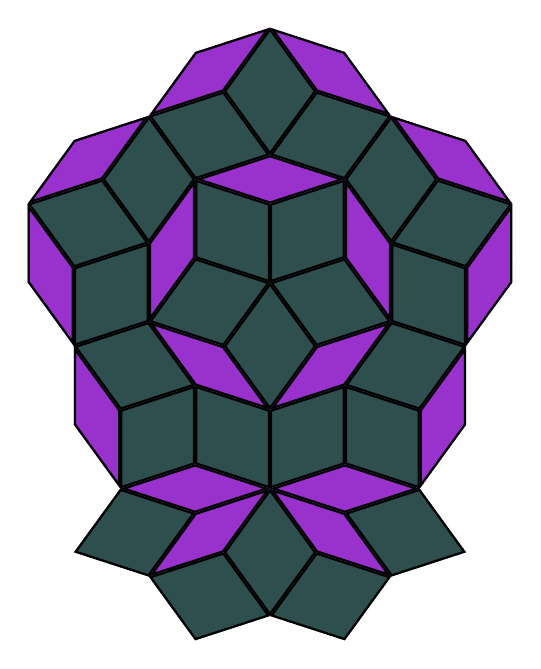
\begin{tikzpicture}[
  every rhombus/.style={
    draw=black,
    ultra thick,
  },
  every thin rhombus/.style={
    every rhombus/.try,
    fill=thinRhombus,
  },
  every thick rhombus/.style={
    every rhombus/.try,
    fill=thickRhombus,
  },
  every circle arc/.style={
    draw=circleArc
  },
  every long arc/.style={
    draw=longArc
  }
]
\pic[rotate=18,thick rhombus,name=a0];
\foreach[evaluate=\k as \kmo using int(\k-1)] \k in {1,...,4} 
{
  \pic[thick rhombus,name=a\k,align with={a\kmo} along A];
}
\foreach \k in {0,...,4} 
{
  \pic[thin rhombus,name=b\k,align with={a\k} along B];
  \pic[thick rhombus,name=c\k,align with={b\k} along A];
  \pic[thick rhombus,name=d\k,align with={b\k} along a];
  \pic[thick rhombus,name=e\k,align with={c\k} along A];
  \foreach \l/\a in {{0/b},{1/B}}
    \pic[thin rhombus,name=f\k\l,align with={e\k} along \a];
}
\pic[thin rhombus,name=g0,align with={f10} along a];
\pic[thin rhombus,name=g1,align with={f21} along A];
\foreach \l/\a in {{0/a},{1/A}}
  \pic[thick rhombus,name=h\l,align with={g\l} along \a];
\pic[thick rhombus,name=i,align with=g0 along B];
\foreach \l/\a in {{0/a},{1/A}}
  \pic[thick rhombus,name=j\l,align with=i along \a];
\end{tikzpicture}
\end{example}

The tiles can be styled, either directly or using various keys.
Each tile has the following styles applied (in this order):
%
\begin{enumerate}
\item \Verb+every Penrose Tile+
\item \Verb+every <name>+
\item \Verb+pic actions+
\end{enumerate}
%
The \Verb+pic actions+ are any actions given directly to the tile, as in \Verb+\pic[draw,thin rhombus];+.
The kite, dart, and rhombus tiles also have arcs drawn on them and these are styled as \Verb+every circle arc+ and \Verb+every long arc+.
The names come from the way the arcs look on the rhombus shapes.

One other point is important to note about the tiles.
They are actually clipped against themselves.
This ensures that the tiles do not overstep their bounds and so when placed alongside each other then they do not go over each other.
In practical terms, this means that if drawn then the line width is half that which might be expected (but when placed next to another tile, the two halves combine to the expected width).

\subsection{Placing Tiles Automatically}

There is a way to specify a Penrose tiling using \emph{Lindenmayer systems}.
In brief, this takes a golden triangle or gnomon (or one of the reverse ones) and repeatedly decomposes it into smaller triangles and gnomon.
Once a desired level has been reached, the resulting triangles and gnomon are glued together in pairs to create either darts and kites or rhombuses (of both types).
This library contains an implementation of this both for kites and darts and for rhombuses.

The user command is:
%
\begin{verbatim}
\PenroseDecomposition{<type>}{<level>}{<seed>}
\end{verbatim}
%
where \Verb+<type>+ is one of:
%
\begin{itemize}
\item \Verb+kite+ for the kite and dart tiling,
\item \Verb+rhombus+ for the rhombus tiling,
\item \Verb+ktriangle+ for the triangular decomposition used to form the kite and dart tiling but with the individual triangles
\item \Verb+rtriangle+ for the triangular decomposition used to form the rhombus tiling but with the individual triangles.
\end{itemize}

The \Verb+<seed>+ is a ``word'' that will be used to initiate the Lindenmayer system.
The key letters in the alphabet are \Verb+T+, \Verb+t+, \Verb+G+, and \Verb+g+.

The \Verb+<level>+ controls how far to take the iteration.
The code is not particularly optimised for speed, and once \Verb+<level>+ gets to about \(5\) or \(6\) then we are at the ``make a cup of tea while compiling'' stage, depending on the processor.

\begin{example}
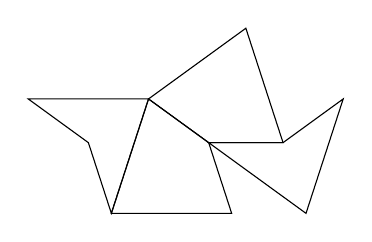
\begin{tikzpicture}[
  every Penrose tile/.style={draw},
  Penrose step=4cm,
]
\PenroseDecomposition{kite}{2}{T}
\end{tikzpicture}
\end{example}

The same styling keys as for the \Verb+pic+ tiles apply, together with some additional ones.
These allow styling the tiles by their number: a count is kept of the number of tiles and each tile knows its own number.
Specifically, two keys are tried:
%
\begin{enumerate}
\item \Verb+Penrose tile <number>+, and
\item \Verb+Penrose tile={<number>}{<total>}+
\end{enumerate}
%
A word of warning is in order on the second of these.
The \Verb+<total>+ is not guaranteed to be correct.
It is done by a quick count at the start of the process and counts those letters which \emph{might} result in a rendered tile.
Not every letter in the resulting word actually does.
Nevertheless, this can be used to style a tile based on what proportion of tiles have been rendered.

Lastly, \Verb+Penrose step+ is used to control the size of the resulting picture.

\begin{example}
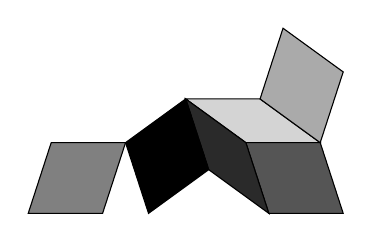
\begin{tikzpicture}[
  every Penrose tile/.style={draw},
  Penrose step=4cm,
  Penrose tile/.code 2 args={
    \pgfmathsetmacro\tint{100*#1/#2}
    \pgfkeysalso{fill=black!\tint}
  }
]
\PenroseDecomposition{rhombus}{3}{T}
\end{tikzpicture}
\end{example}

\section{Deforming Paths}
\label{sec:pathdeform}

This package provides the ability to deform the various tiles.
The various tiles can be built from three paths (labelled \Verb+a+, \Verb+b+, and \Verb+c+) together with their reverses.
By changing these paths, one can get a wide variety of different tiles with the same fundamental matching rules.
Indeed, by using asymmetric paths, the matching rules can be enforced without the need for additional decoration.

Internally, the \Verb+penrose+ library uses the \Verb+spath3+ package for storing and manipulating the paths.

To create a new edge path, use the key \Verb+save Penrose path=<edge>+ where \Verb+<edge>+ is one of \Verb+a+, \Verb+b+, or \Verb+c+.
There are no constraints on the size of the path as all paths are scaled and transformed to fit the tiles.
Once the edge paths have been specified, they are welded together into the tiles using the following command:
%
\begin{verbatim}
\MakePenroseTile{<name>}
\end{verbatim}
%
Here, \Verb+<name>+ is one of the names of the tiles.
This has global effect, as does the definition of the edge paths.
Internally, the tile paths are stored as \Verb+spath+ objects (from the \Verb+spath3+ package) so the commands of that package can be used to, for example, make a copy of a tile.
The internal name for a tile path is \Verb+Penrosepathtile<name>+ (no spaces) so can be cloned via:
%
\begin{verbatim}
\CloneSPath{Penrosepathtile<name>}{My Amazing Penrose Tile}
\end{verbatim}
%
and restored with the same command (but names switched).

\begin{example}
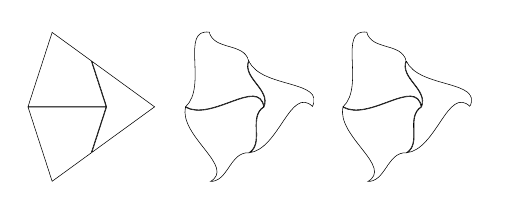
\begin{tikzpicture}
\pic[draw,dart,name=dart];
\pic[draw,kite,align with=dart along c];
\pic[draw,kite,align with=dart along C];
\CloneSPath{Penrosepathtilekite}{Original kite}
\CloneSPath{Penrosepathtiledart}{Original dart}
\path[save Penrose path=a] (0,0) to[out=-30,in=100] (1,0);
\path[save Penrose path=c] (0,0) to[out=-40,in=140] (1,0);
\MakePenroseTile{kite}
\MakePenroseTile{dart}
\pic[xshift=2cm,draw,dart,name=dart];
\pic[draw,kite,align with=dart along c];
\pic[draw,kite,align with=dart along C];
\CloneSPath{Original kite}{Penrosepathtilekite}
\CloneSPath{Original dart}{Penrosepathtiledart}
\pic[xshift=4cm,draw,dart,name=dart];
\pic[draw,kite,align with=dart along c];
\pic[draw,kite,align with=dart along C];
\end{tikzpicture}
\end{example}

With deformed tiles, there is no guarantee that the inner arcs will match up perfectly.

\section{More Examples}

Let's set some aesthetically pleasing shapes.

\begin{example}
\begin{tikzpicture}
\path[save Penrose path=a] (0,0) to[out=-30,in=100] (1,0);
\path[save Penrose path=b] (0,0) to[out=0,in=140] (1,0);
\path[save Penrose path=c] (0,0) to[out=-40,in=140] (1,0);
\MakePenroseTile{thin rhombus}
\MakePenroseTile{thick rhombus}
\MakePenroseTile{golden triangle}
\MakePenroseTile{reverse golden triangle}
\MakePenroseTile{golden gnomon}
\MakePenroseTile{reverse golden gnomon}
\MakePenroseTile{kite}
\MakePenroseTile{dart}
\end{tikzpicture}
\end{example}

Styling the first tile.
Note that as the pattern is formed by repeating two different initial seeds \(5\) times, there are \(10\) ``first tiles'' in each overall pattern.

\begin{example}
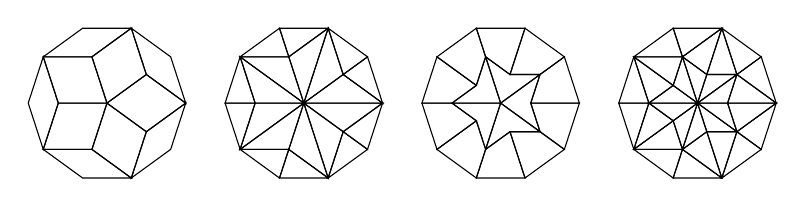
\begin{tikzpicture}[
  every Penrose tile/.style={draw},
  Penrose tile 1/.style={fill=yellow},
]
\foreach \tp/\pos in {rhombus/0cm,rtriangle/2.5cm,kite/5cm,ktriangle/7.5cm}
{
\begin{scope}[xshift=\pos]
\foreach[evaluate=\k as \mk using {\k+Mod(\k,2)},evaluate=\k as \ax using {Mod(\k,2) == 0 ? "T" : "t"}] \k in {0,...,9} {
  \begin{scope}[rotate=\mk*36]
  \PenroseDecomposition{\tp}{1}{\ax}
  \end{scope}
}
\end{scope}
}
\end{tikzpicture}
\end{example}

A more detailed decomposition, with more and more tinting applied to teach tile.
Roughly half of the counted tiles are rendered, and the ordering in which they are rendered is not at first an obvious one (though it is in general from ``outside in'').

Note that the key \Verb+tint fill colour+ is not a TikZ native.
It is defined as:

\begin{verbatim}
\makeatletter
\tikzset{
  tint fill colour/.code={%
    \edef\@temp{%
      \def\noexpand\tikz@fillcolor{\tikz@fillcolor!#1}%
      \noexpand\tikz@addoption{\noexpand\pgfsetfillcolor{\tikz@fillcolor!#1}}%
    }%
    \@temp
  }
}
\makeatother
\end{verbatim}

\begin{example}
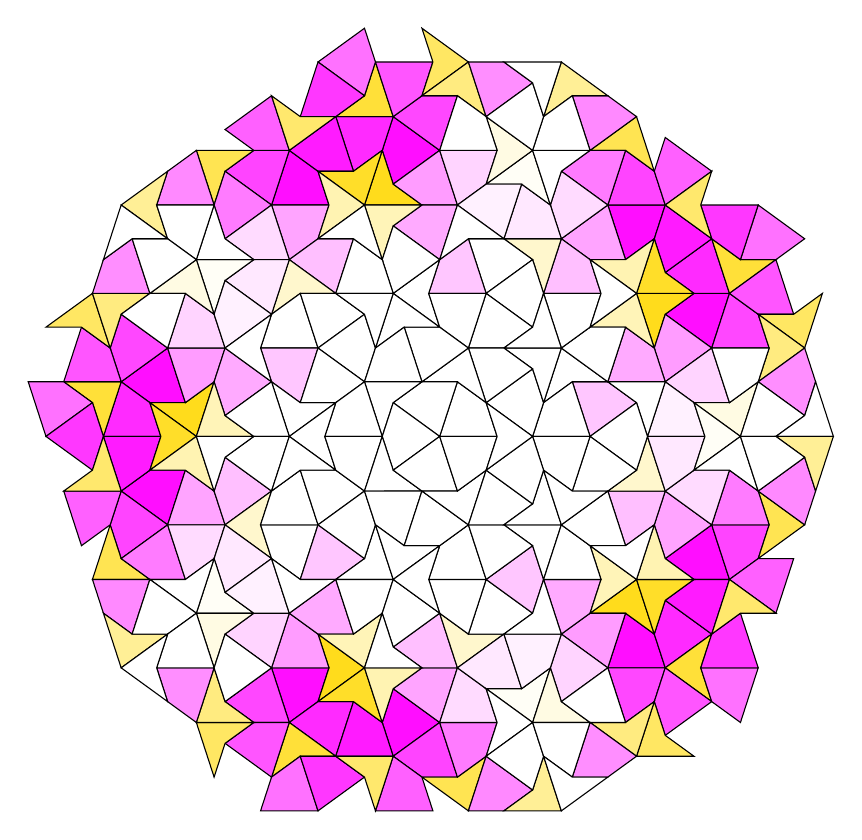
\begin{tikzpicture}[
  every Penrose tile/.style={draw},
  every kite/.style={fill=reverseGoldenTriangle},
  every dart/.style={fill=goldenTriangle},
  Penrose tile/.code 2 args={
    \pgfmathsetmacro\tint{100*(1 - 1.5*#1/#2))}
    \pgfkeysalso{tint fill colour=\tint}
  }
]
\foreach[evaluate=\k as \mk using {\k+Mod(\k,2)},evaluate=\k as \ax using {Mod(\k,2) == 0 ? "T" : "t"}] \k in {0,...,9} {
  \begin{scope}[rotate=\mk*36]
  \PenroseDecomposition[Penrose step=5cm]{kite}{4}{\ax}
  \end{scope}
}
\end{tikzpicture}
\end{example}

An example with ``manual placement''.

\begin{example}
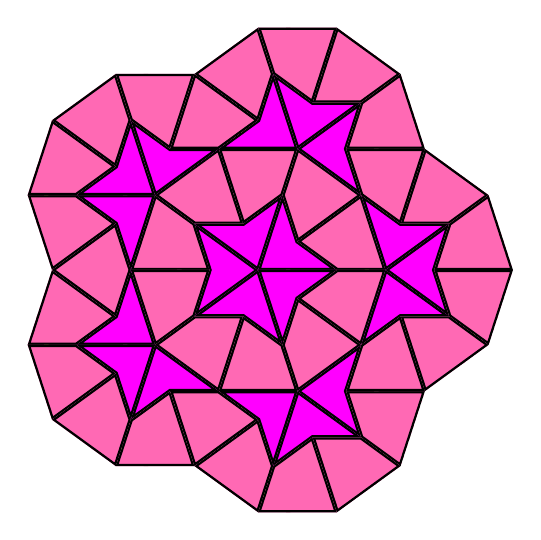
\begin{tikzpicture}[
  every Penrose pic/.style={
    draw=black,
    ultra thick,
  },
  every kite/.style={
    fill=kite,
  },
  every dart/.style={
    fill=dart,
  },
  every circle arc/.style={
    draw=circleArc
  },
  every long arc/.style={
    draw=longArc
  }
]
\pic[dart,name=a0];
\foreach[evaluate=\k as \kmo using int(\k-1)] \k in {1,...,4} {
  \pic[dart,name=a\k,align with={a\kmo} along a];
}
\foreach \k in {0,...,4} {
  \foreach \l/\e/\ee in {0/c/a,1/C/A} {
    \pic[kite,name=b\l\k,align with={a\k} along \e];
    \pic[dart,name=c\l\k,align with={b\l\k} along \ee];
    \pic[kite,name=d\l\k,align with={c\l\k} along \e];
  }
  \pic[kite,name=e\k,align with={c0\k} along C];
  \pic[dart,name=f\k,align with={c0\k} along a];
  \foreach \e in {c,C} {
    \pic[kite,name=g\k,align with={f\k} along \e];
  }
}
\end{tikzpicture}
\end{example}


The decomposition rules for the Lindenmayer system can be illustrated by drawing each tile together with the result of one decomposition superimposed on top.

\begin{example}
\foreach \ax in {T,t,G,g} {

\begin{tikzpicture}
\foreach \tp/\pos in {rhombus/0cm,rtriangle/2cm,kite/4cm,ktriangle/6cm}
{
\begin{scope}[xshift=\pos]
  \PenroseDecomposition[every path/.style={draw=red,ultra thick}]{\tp}{0}{\ax}
  \PenroseDecomposition[every path/.style={fill=gray!50,fill opacity=.5,draw=black}]{\tp}{1}{\ax}
\end{scope}
}
\end{tikzpicture}

}
\end{example}

The tiles can make interesting forms by themselves.

\begin{example}
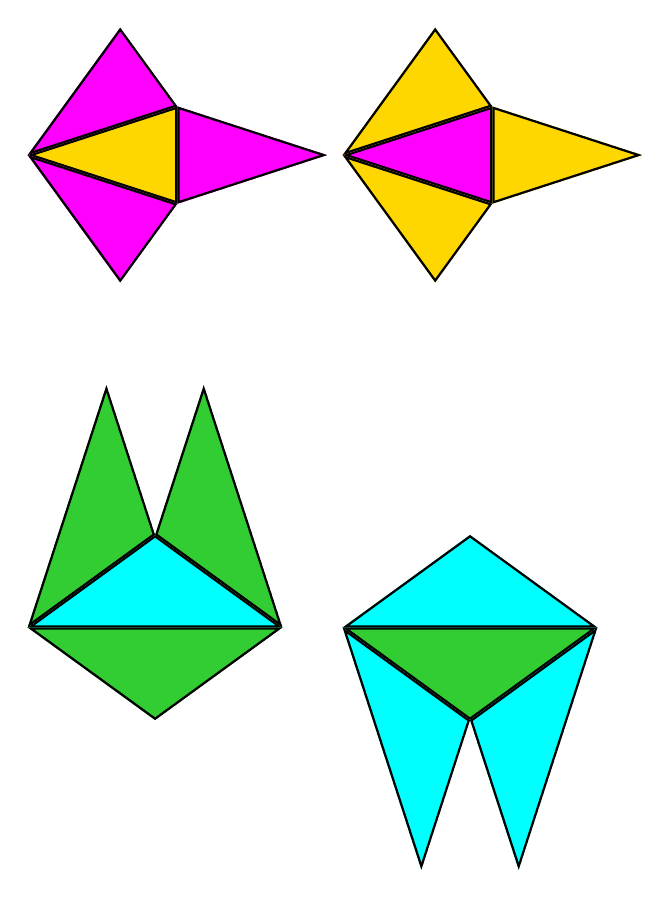
\begin{tikzpicture}[
  scale=2,
  every Penrose pic/.style={
    transform shape,
  },
  every golden triangle/.style={
    draw=black,
    ultra thick,
    fill=goldenTriangle,
  },
  every reverse golden triangle/.style={
    draw=black,
    ultra thick,
    fill=reverseGoldenTriangle,
  },
  every golden gnomon/.style={
    draw=black,
    ultra thick,
    fill=goldenGnomon,
  },
  every reverse golden gnomon/.style={
    draw=black,
    ultra thick,
    fill=reverseGoldenGnomon,
  },
]
\pic[golden triangle,name=a];
\pic[reverse golden triangle,align with=a along a];
\pic[reverse golden triangle,align with=a along b];
\pic[reverse golden triangle,align with=a along c];
\begin{scope}[xshift=2cm]
\pic[reverse golden triangle,name=a];
\pic[golden triangle,align with=a along A];
\pic[golden triangle,align with=a along B];
\pic[golden triangle,align with=a along C];
\end{scope}
\begin{scope}[yshift=-3cm]
\pic[golden gnomon,name=a];
\pic[reverse golden gnomon,align with=a along C];
\pic[reverse golden gnomon,align with=a along b];
\pic[reverse golden gnomon,align with=a along A];
\begin{scope}[xshift=2cm]
\pic[reverse golden gnomon,name=a];
\pic[golden gnomon,align with=a along c];
\pic[golden gnomon,align with=a along B];
\pic[golden gnomon,align with=a along a];
\end{scope}
\end{scope}
\end{tikzpicture}
\end{example}

\begin{example}
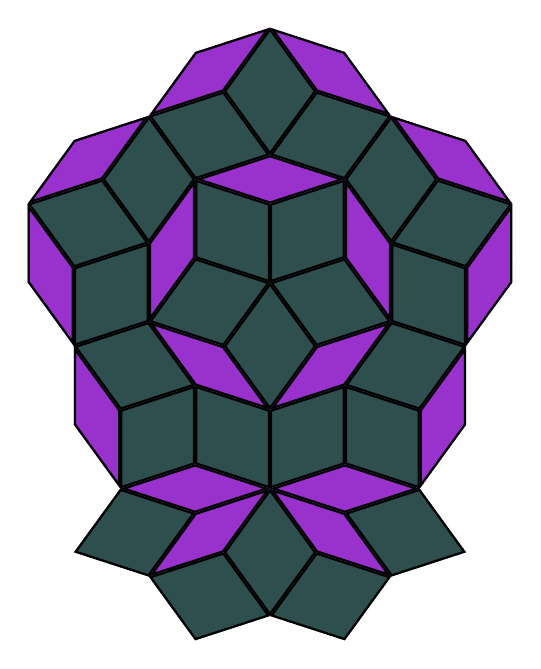
\begin{tikzpicture}[
  every rhombus/.style={
    draw=black,
    ultra thick,
  },
  every thin rhombus/.style={
    every rhombus/.try,
    fill=thinRhombus,
  },
  every thick rhombus/.style={
    every rhombus/.try,
    fill=thickRhombus,
  },
  every circle arc/.style={
    draw=circleArc
  },
  every long arc/.style={
    draw=longArc
  }
]
\pic[rotate=18,thick rhombus,name=a0];
\foreach[evaluate=\k as \kmo using int(\k-1)] \k in {1,...,4} 
{
  \pic[thick rhombus,name=a\k,align with={a\kmo} along A];
}
\foreach \k in {0,...,4} 
{
  \pic[thin rhombus,name=b\k,align with={a\k} along B];
  \pic[thick rhombus,name=c\k,align with={b\k} along A];
  \pic[thick rhombus,name=d\k,align with={b\k} along a];
  \pic[thick rhombus,name=e\k,align with={c\k} along A];
  \foreach \l/\a in {{0/b},{1/B}}
    \pic[thin rhombus,name=f\k\l,align with={e\k} along \a];
}
\pic[thin rhombus,name=g0,align with={f10} along a];
\pic[thin rhombus,name=g1,align with={f21} along A];
\foreach \l/\a in {{0/a},{1/A}}
  \pic[thick rhombus,name=h\l,align with={g\l} along \a];
\pic[thick rhombus,name=i,align with=g0 along B];
\foreach \l/\a in {{0/a},{1/A}}
  \pic[thick rhombus,name=j\l,align with=i along \a];
\end{tikzpicture}
\end{example}


\end{document}

% Local Variables:
% tex-output-type: "pdf18"
% End:
